\chapter{Solução Proposta}
\label{ch:4}

Neste capítulo, apresentaremos os componentes desenvolvidos para a realização dos objetivos propostos, bem como, detalhes de implementação considerados importantes para o melhor entendimento técnico do mecanismo. 

Também será mostrada uma análise do processo de gerenciamento automático, tendo em vista as idéias do ciclo PDCA, apresentado na Seção \ref{sec:pdca} deste trabalho. Essa análise irá relacionar as etapas definidas no ciclo com os sub-processos definidos pelo mecanismo.

\section{Visão Geral}
O contexto ao qual este trabalho está inserido, foi apresentado no capítulo \ref{ch:3}, através da plataforma DSOA, que provê um ambiente de composição dinâmica baseado em componentes orientados a serviços, com percepção de requisitos não-funcionais mapeados em atributos de qualidade. 

Porém, o estado atual da plataforma não dá suporte ao gerenciamento e monitoramento do provedor de serviços. O provedor basicamente define um conjunto de atributos de qualidade, que são utilizados pelos consumidores na seleção de serviço e na elaboração de contratos.

Atacar tais limitações mostra-se relevante, a medida que a qualidade do serviço é um fator chave tanto seleção do provedor quanto na manutenção dos contratos.

Buscando resolver esse problema, o objetivo deste trabalho é especificar e construir um mecanismo de gerenciamento automático de provedores de serviço, focado na prevenção de possíveis quebras de contrato. 

Para isso, a plataforma deve ser capaz de monitorar e adaptar dinamicamente o provedor de serviços, em função do contexto em que o mesmo executa.


\section{Arquitetura}
\label{sec:arch_prop}

Como vimos na Seção anterior, a plataforma DSOA, não prevê o gerenciamento do provedor de serviços com base em atributos de qualidade, deste modo, propomos uma estender a plataforma para suprir tais necessidades.

Para isso, foram desenvolvidos e implantados 2 módulos à plataforma. Um módulo de monitoração de recursos de hardware e um módulo de gerenciamento de provedores de serviços, ver Figura \ref{fig:proposal}.

O módulo de monitoração de recursos consiste em um sensor que captura informações referentes ao estado dos recursos da máquina. É instrumentado através de JMX e foi disponibilizado como um serviço da plataforma. 

O módulo de gerenciamento de provedor de serviço estende um \textit{container} fornecendo suporte a reconfiguração dinâmica de serviços. A reconfiguração é baseada em atributos de qualidade e no contexto em que o provedor executa.

A figura \ref{fig:proposal} destaca onde o trabalho desenvolvido esta situado na plataforma DSOA.

\begin{figure}[htp]
\centering
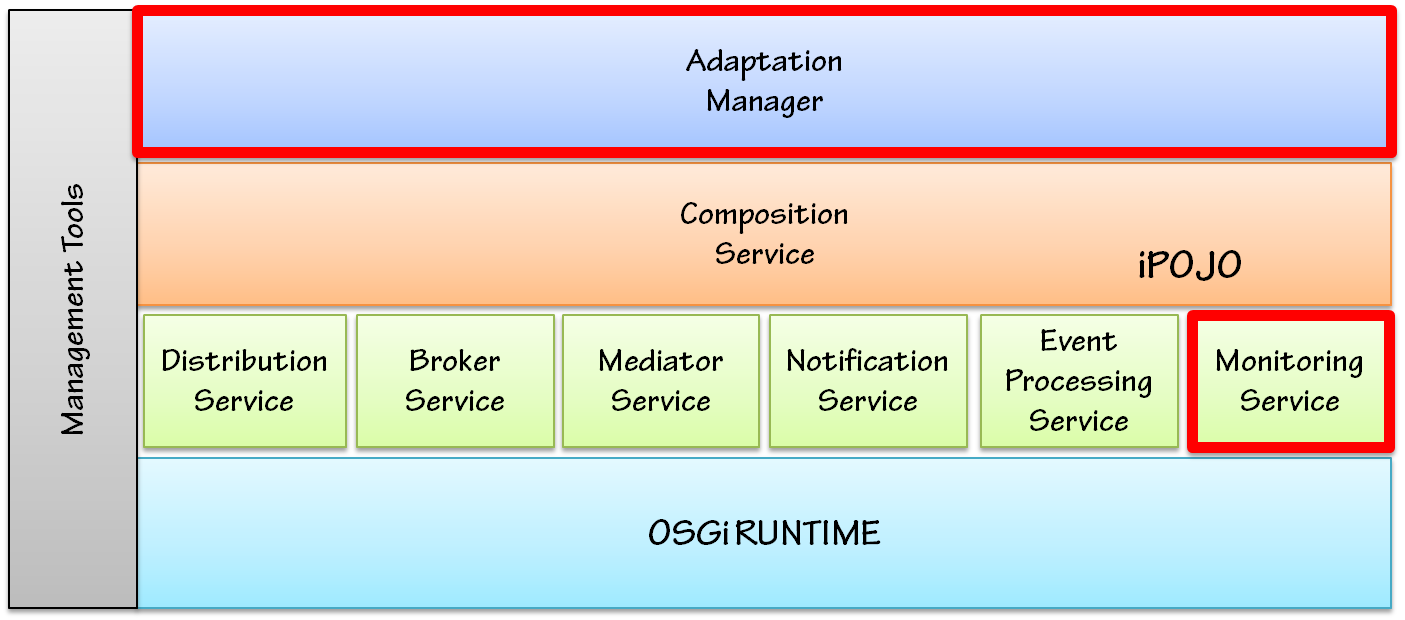
\includegraphics[width=13cm]{chapters/chapter4/dsoa-provider-manager.png}
\caption[Visão Geral da Proposta na Arquitetura]{Visão Geral da Proposta na Arquitetura.}
\label{fig:proposal}
\end{figure}

A combinação destes 2 módulos, junto aos serviços providos pela plataforma, surge como uma solução para o problema de gestão de provedores de serviço. Detalharemos seu funcionamento e arquitetura nas próximas seções.


\subsection{Módulo de Monitoração de Recursos}

Conforme o Capítulo \ref{ch:3}, um elemento importante de um sistema de monitoração corresponde a figura dos sensores. Sensores são responsáveis por coletar dados referentes aos recursos monitorados. E na plataforma DSOA, estão representados pelos serviços de monitoração. 

Originalmente a plataforma suporta um conjunto de sensores responsáveis pela coleta de dados referente a qualidade do serviço. Contudo, do ponto de vista do provedor, 2 fatores impactam diretamente na qualidade: a demanda e a limitação dos recursos de hardware e software~\cite{ye2011models}. 

Neste contexto, é vital que os recursos sejam monitorados, de forma a evitar que o consumo elevado degrade a qualidade do serviço provido, prevenindo eventuais quebras de contratos.

Essa necessidade nos levou a proposição de um novo conjunto de sensores, com a finalidade coletar dados relacionados ao contexto de execução do serviço, em termos de consumo de recursos de hardware, em particular, consumo de CPU e memória. 

Esse conjunto de sensores, foi incorporado à plataforma DSOA, através do serviço de monitoração de recursos (\textit{Resource Monitoring Service}), que é parte integrante do serviço de monitoração (\textit{Monitoring Service}), conforme a Figura \ref{fig:resc_module}.

\begin{figure}[htp]
\centering
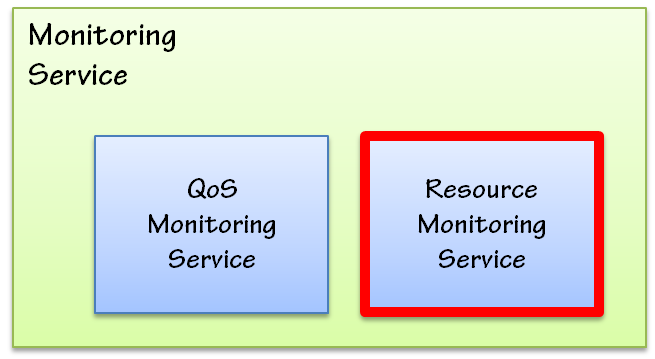
\includegraphics[width=9cm]{chapters/chapter4/monitoring-service.png}
\caption[Resource Monitoring Service]{Resource Monitoring Service.}
\label{fig:resc_module}
\end{figure}

Como foi dito na Seção \ref{sec:arch_prop}, o serviço de monitoração de recursos foi desenvolvido utilizando JMX para realizar a coleta de dados acerca dos recursos da máquina. Esse processo é realizado através de uma técnica de \textit{polling}~\cite{patterson2005organizacao} sobre os dados de memória e utilização de CPU.

Os dados do monitoramento são enviados, através da figura de eventos, ao serviço de processamento de eventos (\textit{Event Processing Service}), que gera notificações ao gerenciador de adaptação (\textit{Adaptation Manager}) quando o provedor encontra-se em um ``Estado de Alerta''.

Um estado de alerta pode ser visto como uma iminência de quebra de contrato. Onde o provedor chegou a um ponto crítico de utilização dos recursos e logo não poderá garantir a qualidade devida, necessitando de adaptar-se ao novo contexto de execução.

\subsection{Módulo de Gerenciamento de Provedor}
\label{subsec:qos_provider}
Em linhas gerais, um processo de garantia de qualidade envolve um ciclo de atividades compreendendo além da coleta e análise dados, uma intervenção que representa uma ação ou conjunto de ações realizadas com base nessa análise. 

Na plataforma DSOA, as etapas de coleta e análise são tratadas respectivamente pelo serviço de monitoração e pelo serviço de processamento de eventos. A ação é de responsabilidade do gerente de adaptação, que no contexto do provedor de serviços, atualmente não realiza nenhum tipo de tratamento.

Deste modo, verificou-se a necessidade de estender o gerente de adaptação para atuar também no contexto do provedor, uma vez que, o monitoramento de recursos é restrito apenas à identificação de estados de alerta.

Assim, o módulo de gerenciamento do provedor (\textit{QoS Provider Manager}) implementa uma extensão do \textit{container} com o  objetivo de permitir que este se adapte dinamicamente, em função do estado atual de consumo de recursos e da qualidade do serviço provido. Essa extensão é apresentada na Figura \ref{fig:adapt_module}.


\begin{figure}[htp]
\centering
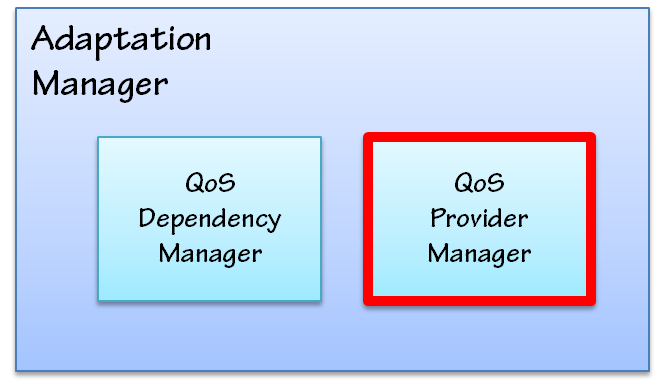
\includegraphics[width=9cm]{chapters/chapter4/adaptation-manager.png}
\caption[QoS Provider Manager]{QoS Provider Manager.}
\label{fig:adapt_module}
\end{figure}

O módulo de gerenciamento do provedor é capaz de adaptá-lo a seu contexto de execução, visando manter a qualidade de serviço, através do gerenciamento das políticas de criação de instâncias.

Em ~\cite{volter2005remoting}, temos um capítulo dedicado ao gerenciamento de ciclo de vida dos objetos remotos. Onde são apresentados diversos cenários de utilização ou limitação de recursos e o padrão de criação de instâncias que melhor se adapta a ele.

A partir disto, definimos um conjunto de políticas para cenários específicos de uso dos recursos. Porém, devido a diversidade enorme de cenários existentes, uma vez que, o uso de recursos é extremamente variável de aplicação para aplicação, a melhor maneira de contemplar a maioria dos casos é disponibilizar a política de criação de instâncias como um serviço. 

Deste modo, abrimos um leque à criação de diversas abordagens de gerenciamento de instâncias, a medida que, a política de criação de instâncias é independente do gerenciador de adaptação.


\section{Aplicação do Ciclo PDCA}
Todo o processo de monitoramento e adaptação será baseado nas etapas definidas pelo ciclo PDCA.

Como vimos na Seção \ref{sec:pdca}, o ciclo foca em manter ou melhorar a qualidade de processos, com base nas informações referentes a sua execução.

\begin{figure}[htp]
\centering
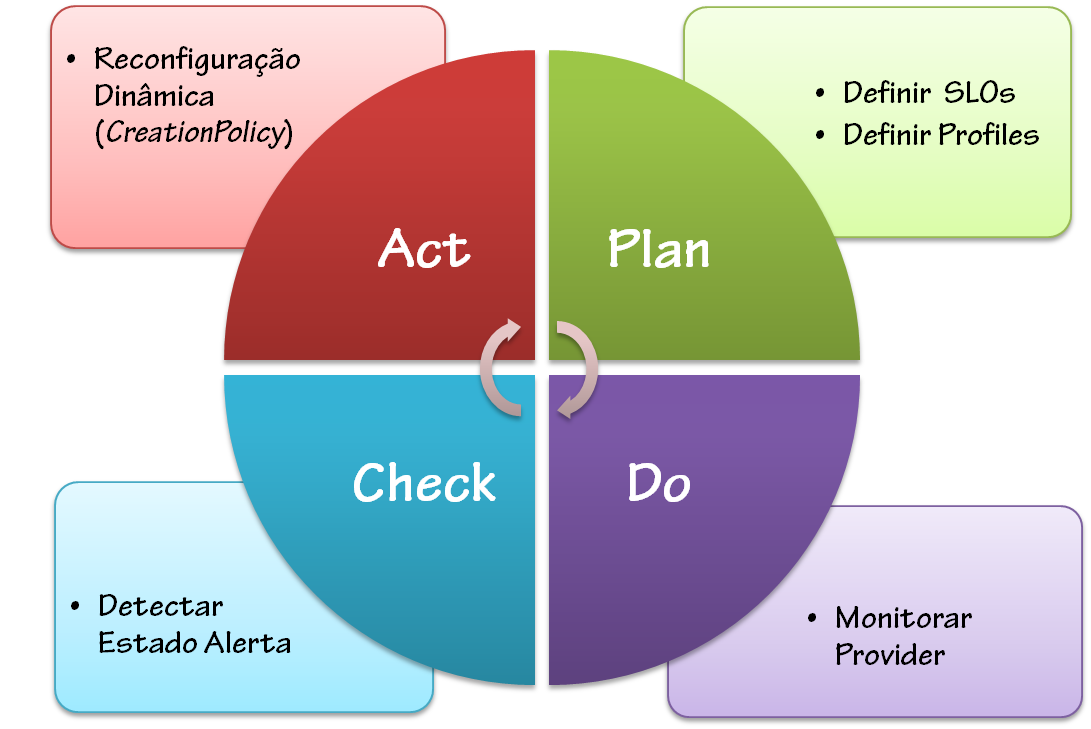
\includegraphics[width=10cm]{chapters/chapter4/pdca_actions.png}
\caption[Aplicação do Ciclo PDCA]{Aplicação do Ciclo PDCA.}
\label{fig:pdcamapping}
\end{figure}

\subsection{\textit{Plan} - Planejar}
Na etapa de planejamento, as metas serão definidas por meio de um documento XML~\cite{xml} que descreve as capacidades que o provedor afirma garantir. Essas propriedades são utilizadas para definir configurações de monitoração (\textit{Monitoring Configuration}), relacionadas a atributos de qualidade do provedor (\textit{e.g} tempo de processamento).

Essas metas são definidas através da \textit{tag} \verb slo , que descreve uma métrica a ser medida, um valor de \textit{threshold} e uma relação de limite(máximo ou mínimo) que o valor do \textit{threshold} pode ultrapassar. Em alguns casos, temos também o identificador da operação provida. Essa informação é útil em casos de configurações de monitoração relacionadas a invocações de determinados métodos do provedor (e.g. \textit{throuhput} de uma operação). Ver Apêndice \ref{subsec:slo}.

Além disso, também são definidos no mesmo XML, métodos que visam atuar sobre estados de alerta, buscando garantir que as capacidades apresentadas sejam devidamente providas.

Esses métodos são descritos pela \textit{tag} \verb profile , que define um conjunto de \verb profiles ~responsáveis por relacionar as configurações de monitoração às políticas de gerenciamento de instâncias, onde cada política de gerenciamento tem por objetivo evitar a degradação da qualidade provida. 

Um  \verb profile ~especifica um conjunto de \verb resources , que assim como os \verb slos , definem uma configuração de monitoração (\textit{monitoring configuration}).

\subsection{\textit{Do} - Executar}
Definidas as metas de qualidade e as políticas de manutenção de recursos (através de \verb slos ~e \verb profiles ), o próximo passo é monitorar o provedor em execução. Cabe ao \textit{Monitoring Service} realizar esta tarefa.

A monitoração de recursos de recursos é de responsabilidade do \textit{Resource Monitoring Service}, que coleta dados referentes ao estado atual da máquina (através de um processo de \textit{polling}) e os envia à central de processamento de eventos.

A monitoração de atributos de qualidade é realizada no próprio gerenciador de adaptação, através da utilização da interceptação das invocações ao serviço.

Um conjunto de técnicas e padrões para captura de atributos relacionados a performance são discutidos em ~\cite{oberortner2011monitoring}~\cite{oberortner2010patterns}.

Deste modo, foi adotado o padrão \textit{QoS Wrapper}~\cite{oberortner2011monitoring} para monitoramento do provedor, uma vez que, este é extremamente simples, não gera um \textit{overhead} elevado e é o que melhor se aplica ao nosso problema.

\subsection{\textit{Check} - Verificar}
A etapa de verificação difere um pouco do processo original, pois ela também ficou responsável por agregar os dados da monitoração. Já que, os dados da monitoração são enviados a cada invocação ao serviço (no caso de dados relacionados a qualidade) ou em intervalos de tempo (no caso de dados relacionados ao estado da máquina).

Além disso, é nesta esta que os estados de alerta são identificados a partir da análise dos dados monitorados em relação aos \verb slos ~e \verb profiles . Essa análise é realizada pelo serviço de processamento de eventos que envia notificações ao gerenciador de adaptação através do serviço de notificação.

\subsection{\textit{Act} - Agir}
A útima fase do ciclo é responsável por garantir o dinamismo da solução através do módulo de gerenciamento do provedor (\textit{QoS Provider Manager}).

O \textit{QoS Provider Manager} recebe notificações referentes ao nível de qualidade do serviço provido e ao estado dos recursos da máquina. E com base nessas informações, reconfigura o serviço visando evitar eventuais quebras de contrato.

A reconfiguração é realizada a partir da modificação da política de criação de instâncias, como foi visto na Seção \ref{subsec:qos_provider}.

\paragraph{}
A figura \ref{fig:dsoa_pcda} mostra onde cada etapa do ciclo está situada na plataforma DSOA.

\begin{figure}[htp]
\centering
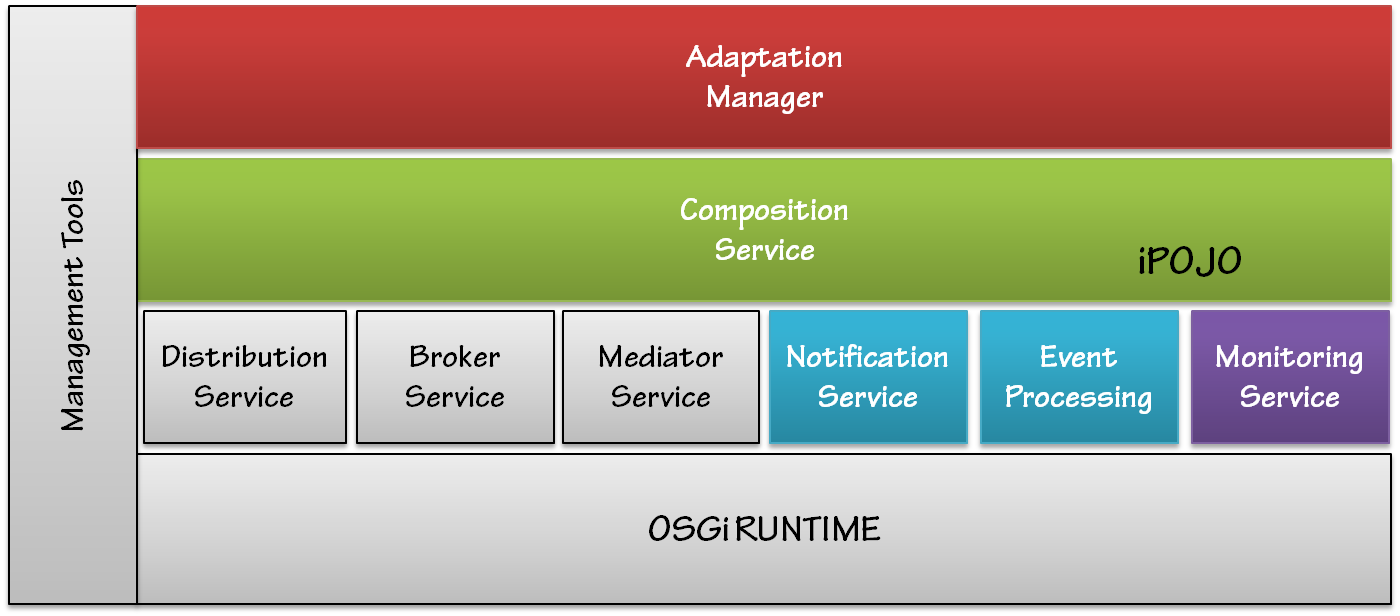
\includegraphics[width=13cm]{chapters/chapter4/pdca_arch_overview.png}
\caption[Componentes da Arquitetura x Fases PDCA]{Componentes da Arquitetura x Fases PDCA.}
\label{fig:dsoa_pcda}
\end{figure}


\section{Avaliação Funcional}
\label{sec:validation}

Para avaliar o mecanismo proposto, utilizamos a ferramenta JMeter~\cite{jmeter} para simulação de carga, através de requições. O ambiente de experimentos contou com o maquinário descrito na Tabela \ref{tab:labs}.

\begin{table*}[htp]
\begin{supertabular}[]{|l|l|l|l|}
\hline
\textbf{Máquina} & \textbf{S.O.} & \textbf{Mémoria RAM} & \textbf{Processador}\\\hline
Máquina 1 & Windows 7 Professional & 2G & Intel Core 2 Duo 2.8 Ghz\\\hline
Máquina 2 & Slackware Linux 13.37 & 2G & Intel Dual Core 2.0 Ghz\\\hline
\end{supertabular}
\caption{Configuração do Ambiente de Experimentos}
\label{tab:labs}
\end{table*}

O provedor de serviços roda na \verb máquina ~\verb 2 , enquando os consumidores (gerados pelo JMeter~\cite{jmeter}) executam na \verb máquina ~\verb 1 .